\documentclass{article}[18pt]
\usepackage{../../../../format}
\lhead{A Level Maths - M2}

%File specific Preamble 
\usetikzlibrary{positioning} %Used for diagram at bottom

\begin{document}
\begin{center}
\underline{\huge M2 Notes}
\end{center}
\section{Centres of mass}
\subsection{Centre of mass of a discrete mass distribution}
$$\overline{x}=\frac{\sum m_ix_i}{\sum m_i}$$
\section{Collisions}
\subsection{Impulse and Momentum}
$$I=m(v-u)$$
\subsection{Coefficient of restitution}
$$e=\frac{\textrm{Speed of seperation}}{\textrm{Speed of approach}}$$
This can be rearranged to give in in terms of heights
$$e=\frac{\sqrt{h_2}}{\sqrt{h_1}}$$
\section{Kinematics}
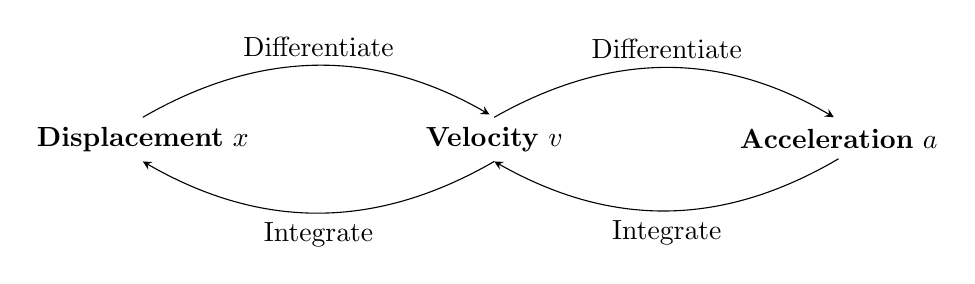
\begin{tikzpicture}
  \node (disp) {\textbf{Displacement} $x$};
  \node[right=2cm of disp] (vel) {\textbf{Velocity} $v$};
  \node[right=2cm of vel] (acc) {\textbf{Acceleration} $a$};
  \draw[-stealth,shorten >= 2pt] (disp.north) to[bend left] node[midway,above] {Differentiate} (vel.north);
  \draw[-stealth] (vel.south) to[bend left] node[midway,below] {Integrate} (disp.south);
  \draw[-stealth,shorten >= 2pt] (vel.north) to[bend left] node[midway,above] {Differentiate} (acc.north);
    \draw[-stealth] (acc.south) to[bend left] node[midway,below] {Integrate} (vel.south);
\end{tikzpicture}
\section{Work, Energy and Power}
$$\textrm{Work}=\textrm{Force}\times\textrm{Distance}$$
$$WD=\mu R\times\textrm{Distance}$$
$$E_K=\frac{1}{2}mv^2$$
$$E_P=mgh$$
$$P=Fv$$


\end{document}